% !TEX encoding = UTF-8 Unicode

\documentclass[12pt,a4j]{ltjsarticle}
\usepackage{semi}
\usepackage{here}

%\title{個人でのVR技術の利用状況} 
%\author{三原巧巳}
%\date{2022年12月14日} 
\begin{document} 

\begin{titlepage}
 \begin{center}
  
    \vspace*{20truept}
    
    {\LARGE 2023年度 卒業論文} 
    
    \vspace*{75truept}
    
    {\Huge } 個人でのVR技術の利用状況
    
    \vspace{85truept}
    
    {\LARGE 指導教員 須田 宇宙 准教授}
    
    \vspace{60truept}
    
    {\LARGE 千葉工業大学 情報ネットワーク学科}
    
    \vspace{15truept}
    
    {\LARGE 須田研究室}
    
    \vspace{70truept}
    
    {\LARGE 1931131 氏名 三原 巧巳 } % 氏名は消さない 学生番号 氏名 名前

    \vspace{70truept}
    
  \end{center}
  \begin{flushright}

    {\LARGE 提出日 2023年1月17日}
  
  \end{flushright}
\end{titlepage}

\setcounter{tocdepth}{3}
% 目次の出力
\tableofcontents
% 表目次
\listoftables
% 図目次
\listoffigures
\clearpage
\pagenumbering{arabic}
\setcounter{page}{1}

%\clearpage

%\tableofcontents
%\clearpage

\section{緒言}
近年,xR(AR,MR,VR)技術の発展により日常生活で技術の使用やコンテンツを見かけることが多くなった.
現在,xR技術は様々な形に変化して利用されている.
AR技術を利用するにはスマートフォンやスマートグラス,MR技術を利用するにはメガネや大きな機械のカメラなどで利用されている.
この2つの技術を用いたコンテンツは,広いスペースや大掛かりな設備を必要としない.

一方,VR技術を利用するには専用のヘッドマウントディスプレイを頭に着用し,視界の全体を覆った上で動き回るため,利用するコンテンツによっては大きな機材や広いスペースを必要とすることがある.
VR技術は主にゲームやアトラクション施設の場で利用されることが多いが,実際に利用できる施設や利用する場面が少ない.
利用される機会が少ないことで,VR技術の普及が低く技術の進化が起こらなくなる.
VR技術の進化がされないことで起こってしまうことは,エンターテイメントの幅が広がらないだけだはなく,現実で行うには危険な実習や現実では起こしにくい体験をすることが困難になるという問題がある.

本研究では,VR技術が普及しない理由として,現在あるVR技術のコンテンツにあると仮説を立て,それを元にVR機器の普及度と,購入されている種類・傾向,および購入していない人に対して購入していない理由などについて調査をし,普及率が低い原因を見つけることを目的としている.


\section{xR技術について}
\subsection{VR技術}
\subsubsection{VR技術とは}
VRとは,「Virtual Reality」の略称であり「仮想現実」とも呼ばれている.
VR専用のヘッドマウントディスプレイやVRゴーグルを装着して,視界全体にコンピューターで作成した空間や世界の映像を映すことで自分が映像の中に入り込んだような体験ができる技術である.
さらにVRの中で自由な移動やものの操作などができ,現実に近い体験から非現実的な体験まで幅広くが扱うことができる.

VRコンテンツを利用するためには,専用のゴーグルが必要になりコンテンツによっては専用のコントローラーなども必要となる.
また体を動かすコンテンツの場合動かすのに十分な空間も必要となる.

VR技術では,主にゲームやエンターテイメントで普及してきたが,幅広い体験をできることから教育や訓練などでも利用されるようになり,近年ではビジネスの分野でも活躍するようになっっている.
ゲームやエンターテイメントの場では,専用のヘッドマウントディスプレイを利用したゲームの世界観を体験しながら遊べるコンテンツがある.
教育や訓練の場では,VRを利用した社会科見学や避難訓練の再現などといったもので利用されている.
ビジネスの場では,VRでの物件の内見やVRでのショッピングなどといったサービスが増えていっている.

\subsubsection{VR技術の歴史}
VR技術のコンセプトは1935年ごろに作家のスタンリー・G・ワインボウムが発表したSF短編小説「Pygmalion’s Spectacles」の中に,ゴーグルを装着すると仮想的に五感を感じ取りながら擬似体験が可能な装置が登場する.

VR技術の研究が始まったのは1960年代頃かである.映画作成者で仮想現実技術のパイオニアであるモートン・ヘイリグが1962年にセンソラマと呼ばれる世界最初期のVR機器が開発された.
センソラマとは図\ref{fig:センソラマ.pdf}のような大型のシステムであり,没入型で多感覚入力が可能というマルチモーダルインターフェースを採用している.

\begin{figure}[h]
\begin{center}
 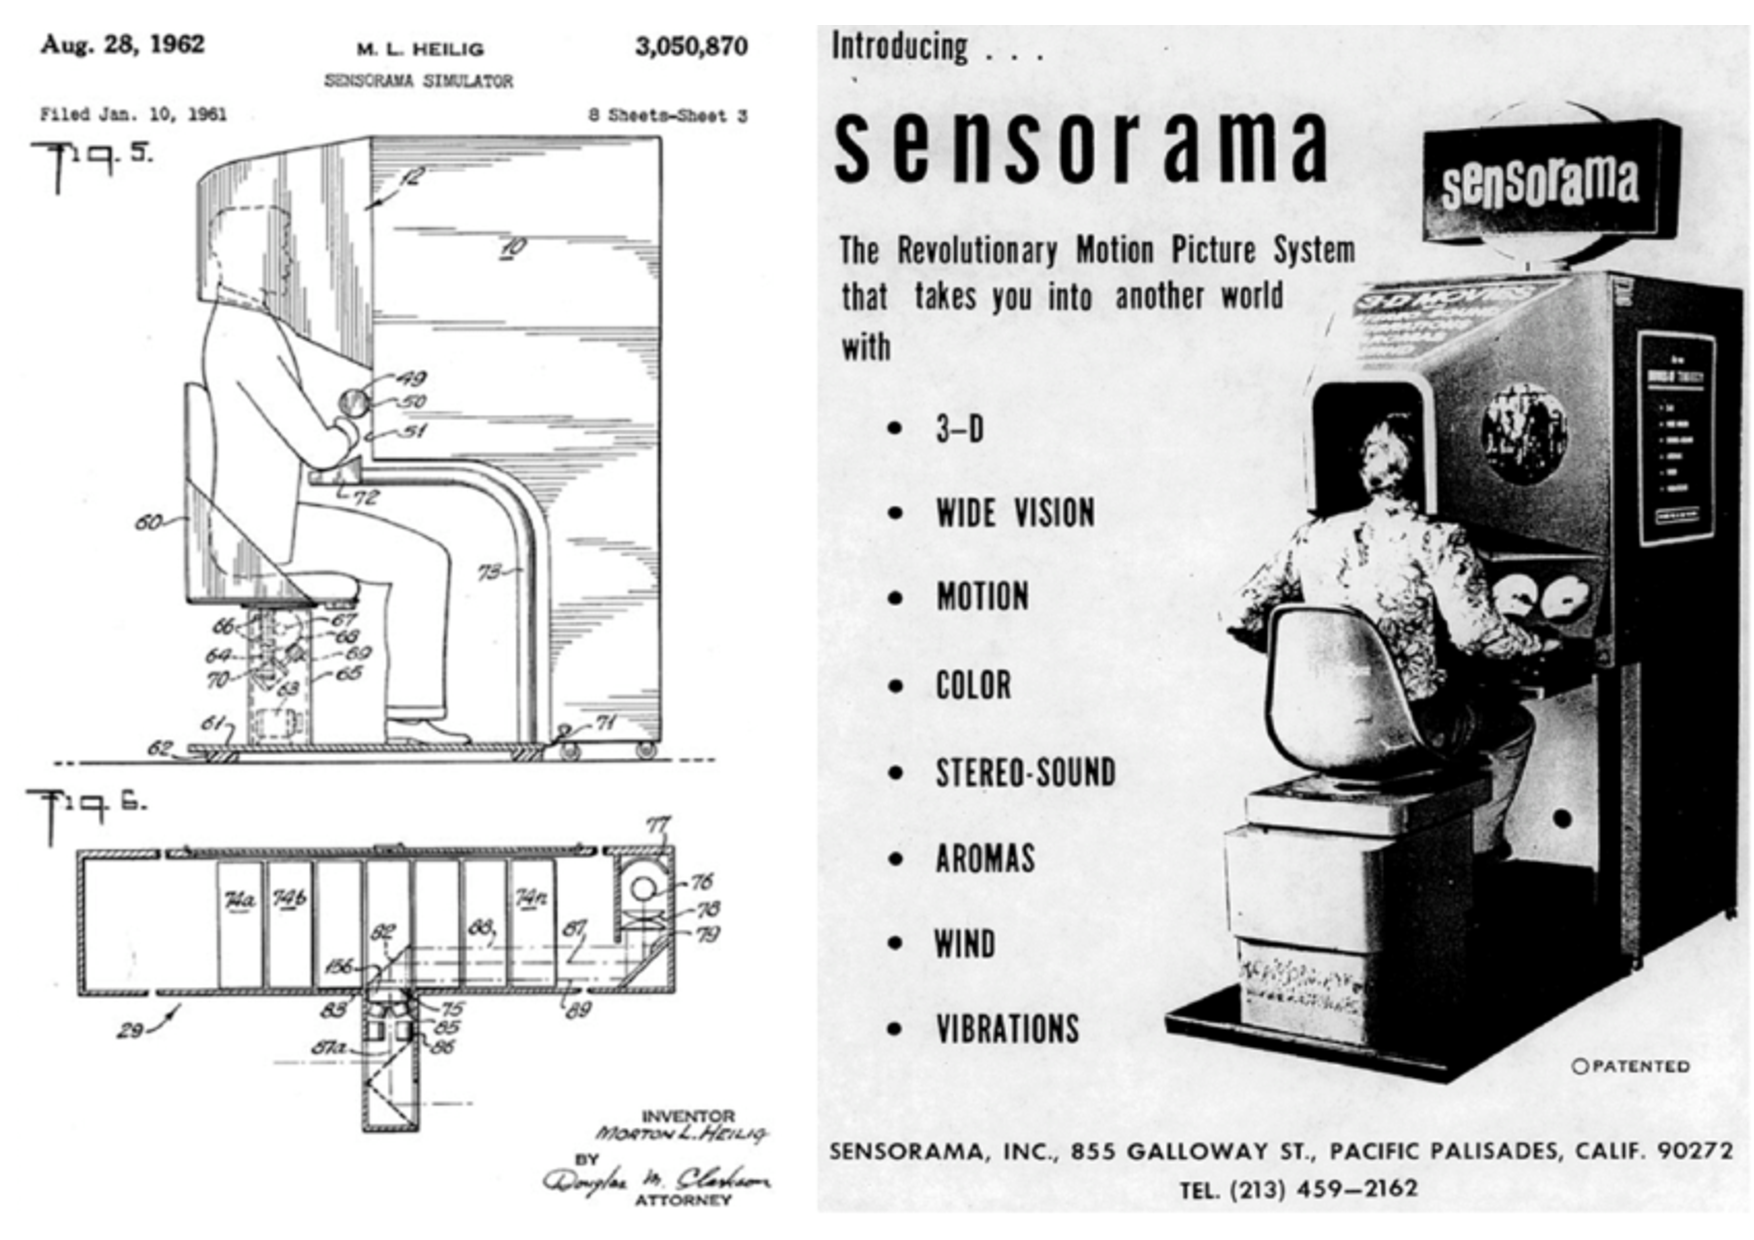
\includegraphics[clip,width=85mm,height=55mm]{センソラマ.pdf}
\end{center}
 \caption{センソラマ}
 \label{fig:センソラマ.pdf}
\end{figure}

その後1968年にユタ大学のアイバン・サザランドは,「ダモクレスの剣」というヘッドマウントディスプレイを開発したが,どちらも実用性が低くかった\cite{VRの概念の登場}.

1990年代前後からVR機器の商用化が始まった.
VPL Research社がRB2(Reality Built dfor 2)というVRを利用したコミュニケーションシステムを発表した.
このシステムは,ヘッドマウントディスプレイを使用した2人が同じVR空間で会話ができる3Dテレビ会議のようなシステムのようなシステムである.
しかし,当時のVR機器は価格が高いだけではなく性能が価格と見合っていないということから一般家庭に普及しなかった.
この商用化から約10年間はVRの第1次ブームと言われている\cite{VRの初の商用化}.

スマートフォンやゲーム機などのハードウェアの進化により2010年代以降にVRが再び注目される\cite{VRの概念の登場}.
スマートフォンでVRを利用したアプリケーションが開発されたり,以前より安価で性能が高くなった機器が出たことから,第1次ブームの時よりも日常的なものになろうとしている.

\subsection{AR技術}
\subsubsection{AR技術とは}
ARとは,「Augmented Reality」の略称であり「拡張現実」とも呼ばれており,現実を仮想的に拡張する技術である.
具体的にはスマートフォンやタブレットなどのカメラを通して現実世界を映し,その上にCG映像や文字情報を重ねることで重ねたデータが実在しているように見える技術である\cite{ARとは}.

ARコンテンツを利用するためには,専用の機材を必要とせずスマートフォンやカメラがついているPCなどで利用することができる.

AR技術は,元々PCで利用されていた技術だったかスマートフォンの技術が進歩したことにより気軽に利用できる技術になった.
スマートフォンで利用できるようになったためエンターテイメントの分野でも活躍するようになった.

\subsubsection{AR技術の歴史}
現在のAR技術の概念の登場は1901年である.
小説家のライマン・フランク・ボームが書いた「The Master Key: An Electrical Fairy Tale」の中で登場した現実の世界にデジタルを重ね合わせる電子ディスプレイの概念を提唱したことが始まりとされている.

1968年にハーバード大学教授であり計算機科学者であったアイバン・サザランドが教え子のボブ・スプロールと共に仮想現実を創り出すヘッドマウントディスプレイ・システム「The Sword of Damocles」を開発した.

\begin{figure}[h]
\begin{center}
 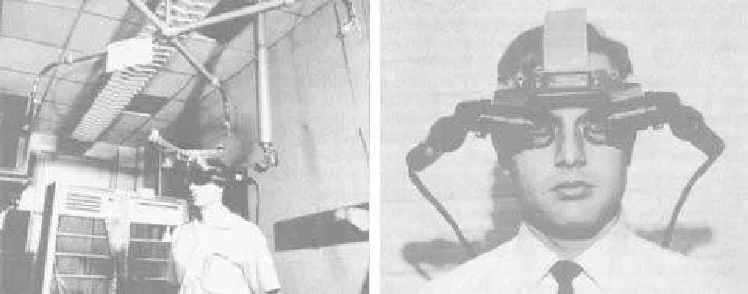
\includegraphics[clip,width=85mm,height=55mm]{The_Sword_of_Damocles.pdf}
\end{center}
 \caption{The\_Sword\_of\_Damocles}
 \label{fig:The_Sword_of_Damocles.pdf}
\end{figure}

図\ref{fig:The_Sword_of_Damocles.pdf}のデバイスを装着することで,ユーザーはCGで作られた環境で仮想体験ができるというシステムである.
しかしこのデバイスは重すぎるため天井から吊り下げて使用するというものになっている.
また,仮想空間で作り出せるものはシンプルな線のみでの構成になっている.

1973年にAR技術は,「Augmented Reality」の前に「Artificial Reality」または「人工現実」として提唱されていた.
この技術はAR技術ではなくVR技術に近いものである.
「Augmented Reality」は1990年にトム・コーデルが名付けた.

1990年代にITによる効率化の影響によりAR技術は急速に進化していった.
1992年にアメリカ空軍で世界初の操作可能のARシステムが開発された.
このシステムは現在のAR技術が持つ基本性能を持っているとされている.
1993年にコロンビア大学のスティーブン・フェイナーがレーザープリンターのメンテナンスのサポートを行うARシステムを発表した.
このシステムはHMDを装着することで,超音波センサーにより検知したレーザープリンターの内部構造情報や修理が必要な箇所がコンピュータグラフィックで表示することができた.
しかし,このシステムは対象物に超音波センサをつけなければいけなかったため実用化はされなかったが,現在の業務用ARシステムのコンセプトを作り出したシステムとなっている.
ここからAR技術は舞台やテレビ,飛行機などにも利用されるようになり急成長していった.

1999年にARアプリケーションを実現するためのライブラリ『ARToolKit』が,当時ワシントン大学HITラボ滞在中だった奈良先端科学技術大学院大学の加藤博一によって高度技術の研究用のC言語ライブラリとして開発された.
1990年代のシステムは高価な位置姿勢計測装置が必要だったが,「単眼カメラ」と「平面マーカー」のみを使って実装するARアプリケーションの開発を可能にしただけでなく,AR技術をより容易に使うことを可能にした.

2000年に入り,携帯端末の性能が向上したことにより様々なARのアプリケーションが誕生し一般に広まった.
2013年にGoogleが発表した「Google Glass」の登場によりグラス型のデバイスが増えていった.
図\ref{fig:Google_Glass.pdf}のように手荷物必要のないハンドフリーかつスタンドアローン型の新しいパソコンとして期待されたが,社会問題と技術問題から一般的な販売は中止になった\cite{ARの歴史}.

\begin{figure}[h]
\begin{center}
 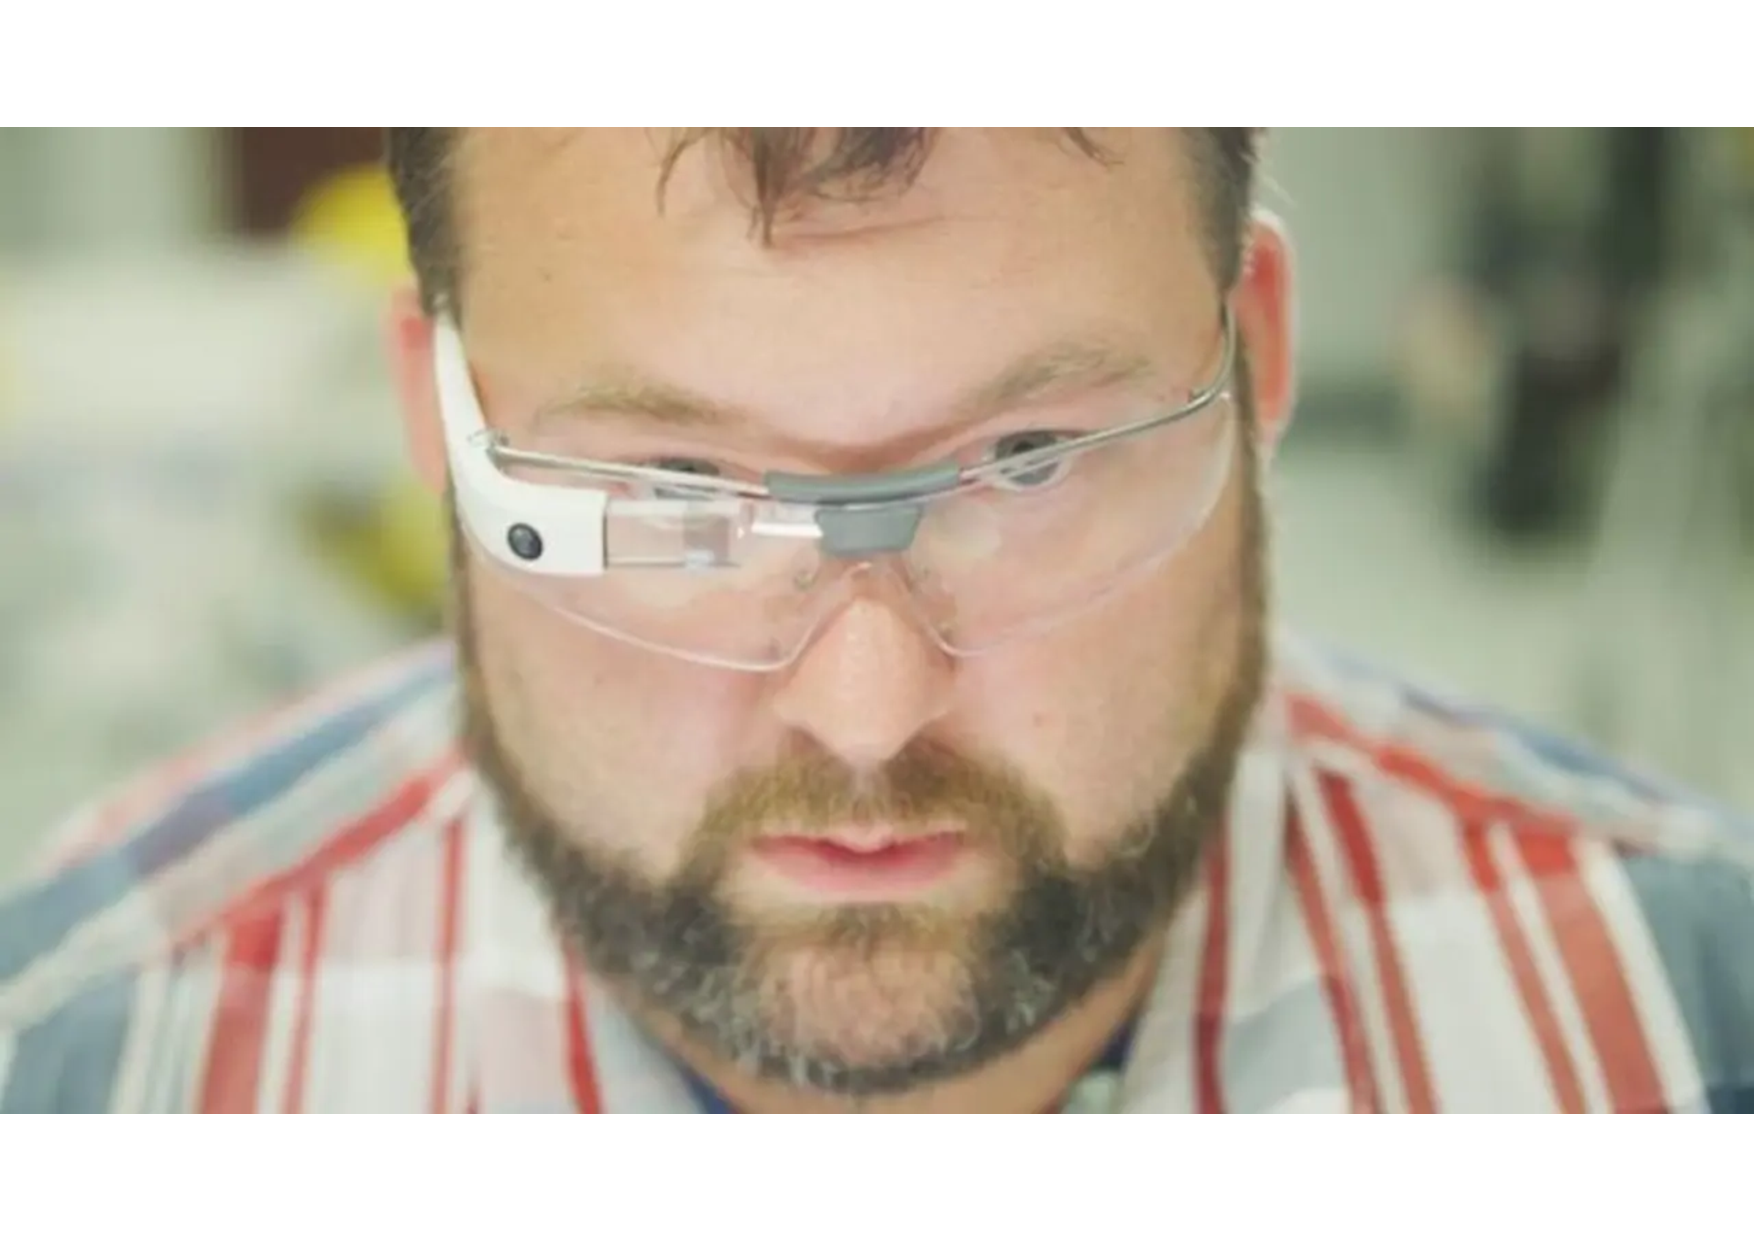
\includegraphics[clip,width=85mm,height=55mm]{Google_Glass.pdf}
\end{center}
 \caption{Google Glass}
 \label{fig:Google_Glass.pdf}
\end{figure}

\subsection{MR技術}
\subsubsection{MR技術とは}
MRとは,「Mixed Reality」の略称であり「複合現実」とも呼ばれいる.
ヘッドマウントディスプレイやカメラで現実世界を認識し,そこに合わせたCG映像や文字情報などを重ねて表示することで現実世界と仮想世界を融合させる技術である.
MR技術では,現実世界の景色も見ることができるため仮想データを見ながら現実世界で体を移動させたり,仮想世界で作成したものを多角的に見ることが可能になる.
MR技術はAR技術と似ているが,AR技術は主体が現実世界でありそこに仮想データの情報だけを表示する技術であり,MR技術は現実世界と仮想世界の融合のため実際にそこにあるかのように現実とかそうが相互作用するようなリアルタイム映像の技術である\cite{MRとは}.

主にMR技術はビジネスの場で使われることが多く,建設現場の完成イメージの確認や研修の再現,医療現場での患者の情報表示などといった場で利用されている.

MR技術を利用するには,ヘッドマウントディスプレイやカメラだけではなく,コンテンツによっては仮想世界で作られたものを映すためのマーカーなども必要となる.

\subsubsection{MR技術の歴史}
MR技術は1994年にトロント大学のP.Milgramによって提唱された.
計算機内に構築される仮想世界と現実世界で強化するという概念を仮想化現実と呼び,現実世界を電子的に強化と増強することを拡張現実と対置した上で両方の要素を取り入れたMRを提唱した.
1997年に「複合現実感システムに関する試験研究」で複合現実感という言葉が登場した.
MR技術の研究は1993年ごろから始まっており,ヘッドマウントディスプレイによる情報提示を活用するという研究だった\cite{MRの歴史1}.

MR技術が市場に流通したのは2015年である.
発表されたものは,スタンドアローン型のヘッドマウントディスプレイで,コントローラーを必要とせずハンドトラッキングと音声入力で操作するものである.
この発表でMR技術は新たな体験をできる機材として市場に認知されるようになった\cite{MRの歴史2}.

その後,機器の軽量化や視線に応じて見ている映像が変化する技術,ホログラムで表示されたものを摘んだりする技術などによってより現実に馴染むことが可能になる機器が登場した.

現在市場に存在するMR機器は3種類のみであり,機器の独自性が高くなっている.


\section{xRのコンテンツについて}
\subsection{VRのコンテンツ}
\subsection{ARのコンテンツ}
\subsection{MRのコンテンツ}
\section{第1回目のアンケート}
\subsection{仮説}
\subsection{内容}
\subsection{結果}
\section{第2回目のアンケート}
\subsection{仮説}
\subsection{内容}
\subsection{結果}
\section{考察}
\section{結言}
\section{謝辞}
\begin{thebibliography}{99}
\bibitem{VR}  ``流行体感から読み解くサービス未来予測 流行予想シリーズ ~VR(バーチャルリアリティ)編~'', https://research-platform.line.me/archives/38203466.html, 2022/9/2参照

\bibitem{VRの概念の登場}  ``VRはいつから普及が始まった?仮想現実の歴史を紐解く'', https://onetech.jp/blog/when-did-vr-become-popular-11526\#VR20, 2023/1/2参照

\bibitem{VRの初の商用化}  ``VRの初商用化は30年前、現代を生きるクリエイターが知っておくべき歴史と必要な視点とは'', https://creatorzine.jp/article/detail/538, 2023/1/2参照

\bibitem{ARとは}  ``AR(拡張現実)とは? 4つの種類とVR・MRとの違いを解説'', https://www.japancv.co.jp/column/4190/, 2023/1/6参照

\bibitem{ARの歴史}  ``AR100年史 |現実を拡張するテクノロジーの誕生と成長を紐解く'', https://note.com/hato\_fun/n/n4ca0e20000cb, 2023/1/6参照

\bibitem{MRとは}  ``MRとは? AR,VRとの違いやビジネスへの活用法を解説'', https://www.digital-transformation-real.com/blog/what-is-mr\#toc-0, 2023/1/6参照

\bibitem{MRの歴史1}  ``複合現実感の歴史と今後の展望'', https://www.jstage.jst.go.jp/article/isciesci/64/9/64_343/\_pdf, 2023/1/6参照

\bibitem{MRの歴史2}  ``MR(Mixed Reality)が産業にもたらす可能性と未来―MRの利活用に向けて'', https://www.pwc.com/jp/ja/knowledge/column/disruptive-technology-insights/disruptive-technology-insight10.html 2023/1/6参照



\end{thebibliography}

\end{document}
